\documentclass[10pt,a4paper]{article}
\usepackage[margin=17mm]{geometry}
\usepackage{fontspec,amsmath,graphicx,xcolor}
\setmainfont{TeX Gyre Termes}
\definecolor{ink}{HTML}{173C58}
\pagestyle{empty}
\setlength{\parindent}{0pt}
\setlength{\parskip}{5pt}
\begin{document}
\begin{center}
{\Large\bfseries\color{ink} AIAA3201 Lab Week 08}\\[3pt]
{\normalsize Sequence Models and Attention Mechanisms}
\end{center}

\textbf{1. Why divide attention scores by $\sqrt{d_k}$?}
Scaled dot-product attention computes
\[
 A=\operatorname{softmax}\!\left(\frac{QK^\top}{\sqrt{d_k}}\right),
 \qquad Y=AV,
\]
where softmax is applied along the key dimension, so each query's weights sum to one.
If the query and key components are independent, zero-mean and unit-variance,
then $\operatorname{Var}(q\cdot k)=d_k$: the standard deviation grows as
$\sqrt{d_k}$. Dividing by this factor keeps the score variance at approximately
one. Without scaling, increasing the key dimension tends to produce larger
score differences and nearly one-hot softmax distributions. The softmax
Jacobian $\partial a_i/\partial e_j=a_i(\delta_{ij}-a_j)$ then becomes small,
weakening gradient flow. Scaling mitigates this saturation and stabilizes
the attention calculation as the dimension changes.

\textbf{2. What pattern appears in the positional encoding heatmap?}
For pair index $k$, $\omega_k=\exp[-2k\log(10000)/d_{\mathrm{model}}]$,
with $\mathrm{PE}(p,2k)=\sin(p\omega_k)$ and
$\mathrm{PE}(p,2k+1)=\cos(p\omega_k)$.
In the actual $100\times128$ heatmap below, low-index dimensions oscillate
rapidly as sequence position changes. Higher-index dimensions have lower
frequencies and longer wavelengths, so their colors vary slowly over the
100 positions. Adjacent dimensions form sine/cosine pairs with the same
frequency and a phase offset. At position zero they alternate between zero
and one; far to the right, the sine channels stay near zero and the cosine
channels near one, producing nearly constant vertical stripes. This
multiscale encoding is added to the input embeddings without changing
their shape. The separate attention heatmap shows row-wise probability
mass; independent random Q and K do not imply a diagonal pattern.

\begin{center}
\begin{minipage}[t]{0.54\linewidth}
\centering
\includegraphics[width=\linewidth,height=50mm,keepaspectratio]{output/positional_encoding.png}\\[-2pt]
{\footnotesize Positional encoding: positions $0$--$99$, 128 dimensions.}
\end{minipage}\hfill
\begin{minipage}[t]{0.44\linewidth}
\centering
\includegraphics[width=\linewidth,height=50mm,keepaspectratio]{output/attention_weights.png}\\[-2pt]
{\footnotesize Attention: 10 queries and keys, $d_k=64$, seed 42.}
\end{minipage}
\end{center}

\textbf{Verification.}
The unchanged official script passed all three mathematical tests and saved
both heatmaps. Independent checks also passed: random rectangular RNN
weights against a scalar reference; attention with multiple batches,
unequal query/key lengths and different value widths; and positional
encoding at nonzero positions, odd/even dimensions, batch broadcasting,
input addition and buffer registration.

\begin{center}
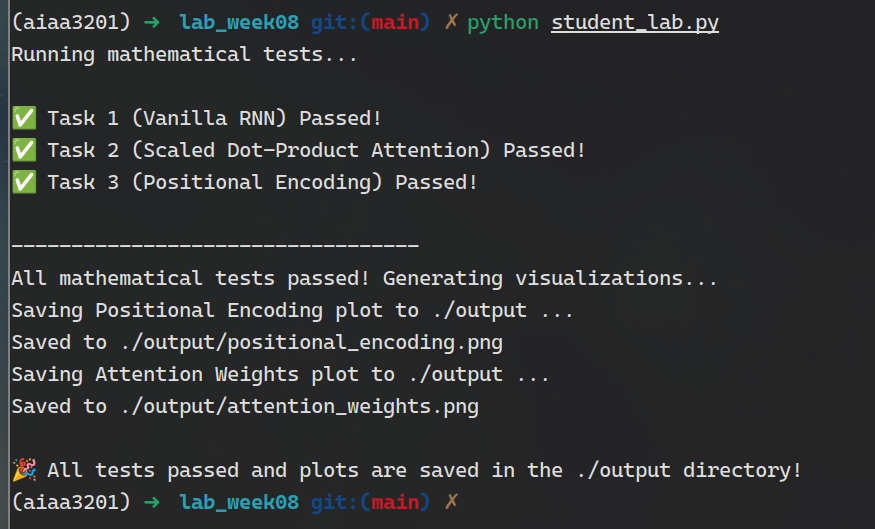
\includegraphics[width=0.94\linewidth,height=70mm,keepaspectratio]{screenshots/verification.png}
\end{center}
\end{document}
